%%%%%%%%%%%%%%%%%%%%%%%%%%%%%%%%%%%%%%%%%%%%%%%%%%%%%%%%%%%%%%%%%%%%%%
% LaTeX Template: Two Column Colour Article
%
% Source: http://www.howtotex.com/
% Feel free to distribute this template, but please keep the
% referal to howtotex.com.
% Date: Feb 2011
% 
%%%%%%%%%%%%%%%%%%%%%%%%%%%%%%%%%%%%%%%%%%%%%%%%%%%%%%%%%%%%%%%%%%%%%%
% How to use overleaf.com: 
%
% You edit the source code here on the left, and the preview on the
% right shows you the result within a few seconds.
%
% You can upload figures, bibliographies, custom classes and
% styles using the files menu.
%
% If you're new to LaTeX, the wikibook is a great place to start:
% http://en.wikibooks.org/wiki/LaTeX
%
%%%%%%%%%%%%%%%%%%%%%%%%%%%%%%%%%%%%%%%%%%%%%%%%%%%%%%%%%%%%%%%%%%%%%%
% adaptions made by wolfgang stoettner mail@stoettner.net
%%%%%%%%%%%%%%%%%%%%%%%%%%%%%%%%%%%%%%%%%%%%%%%%%%%%%%%%%%%%%%%%%%%%%%

%%% Preamble
\documentclass[	DIV=calc,%
							paper=a4,%
							fontsize=11pt,%
							twocolumn]{scrartcl} % KOMA-article class

\usepackage{lipsum}	% Package to create dummy text
\usepackage[english]{babel}	% English language/hyphenation
\usepackage[protrusion=true,expansion=true]{microtype}	% Better typography
\usepackage{amsmath,amsfonts,amsthm} % Math packages
\usepackage[pdftex]{graphicx} % Enable pdflatex
\usepackage{wrapfig} % enable figure wrapping
\usepackage[svgnames]{xcolor} % Enabling colors by their 'svgnames'
\usepackage[hang, small,labelfont=bf,up,textfont=it,up]{caption} % Custom captions under/above floats
\usepackage{epstopdf} % Converts .eps to .pdf
\usepackage{subfig}	% Subfigures
\usepackage{booktabs} % Nicer tables
\usepackage{fix-cm}	% Custom fontsizes
\usepackage{booktabs} % prof. looking tables (www.en.wikibooks.org/wiki/LaTeX/Tables#Professional_tables)

%%% Custom sectioning (sectsty package)
\usepackage{sectsty} % Custom sectioning (see below)
\allsectionsfont{%		% Change font of al section commands
	\usefont{OT1}{phv}{b}{n}%	% bch-b-n: CharterBT-Bold font
	}

\sectionfont{%		% Change font of \section command
	\usefont{OT1}{phv}{b}{n}%	% bch-b-n: CharterBT-Bold font
	}


%%% Headers and footers
\usepackage{fancyhdr} % Needed to define custom headers/footers
	\pagestyle{fancy} % Enabling the custom headers/footers
\usepackage{lastpage}	

% Header (empty)
\lhead{}
\chead{}
\rhead{\today}
% Footer (you may change this to your own needs)
\lfoot{\footnotesize \texttt{Statistics Formulae} \textbullet ~Lind et al. 16ed.}
\cfoot{}
\rfoot{\footnotesize page \thepage\ of \pageref{LastPage}}	% "Page 1 of 2"
\renewcommand{\headrulewidth}{0.0pt}
\renewcommand{\footrulewidth}{0.4pt}
\newcommand{\hformbar}[1]{\vspace{5pt}\hrule\vspace{10pt}} % creates a horizontal bar to separate formulae better; space adaptions can be made centrally here


%%% Creating an initial of the very first character of the content
\usepackage{lettrine}
\newcommand{\initial}[1]{%
     \lettrine[lines=3,lhang=0.3,nindent=0em]{
     				\color{DarkGoldenrod}
     				{\textsf{#1}}}{}}

%%% Title, author and date metadata
\usepackage{titling} % For custom titles

\newcommand{\HorRule}{\color{DarkGoldenrod}%	% Creating a horizontal rule
									  	\rule{\linewidth}{1pt}%
										}

\pretitle{\vspace{-30pt} \begin{flushleft} \HorRule 
				\fontsize{30}{30} \usefont{OT1}{phv}{b}{n} \color{DarkRed} \selectfont 
				}
\title{Statistics Formulae Collection} % Title of your article goes here
\posttitle{\par\end{flushleft}\vskip 0.5em}

\preauthor{\begin{flushleft}\large \lineskip 0.5em \usefont{OT1}{phv}{b}{sl} \color{DarkRed}}
\author{Wolfgang W. Stoettner}	% Author name goes here
\postauthor{\footnotesize \usefont{OT1}{phv}{m}{sl} \color{Black} \hspace{5pt} mail@stoettner.net \par\end{flushleft}\HorRule}

\date{\today} % No date

%%% wws: create a non-indented formula name
\newcommand{\formdesc}[1]{\noindent\textbf{#1}}



%%% Begin document -----------------------------------------------------------------
\begin{document}
\maketitle
\thispagestyle{fancy} 	% Enabling the custom headers/footers for the first page 
% The first character should be within \initial{}
\initial{T}\textbf{he following collection represents an excerpt of the statistics formulae taken from the perennial text book \textit{Lind, Douglas A. et. al. (2015): Statistical Techniques in Business and Economics, Sixteenth edition, New York, NY 2015}.}

\hspace{10pt}

\hformbar
\formdesc{Frequency distributions}
\begin{equation}
\label{frequency distributions}
\end{equation}
\footnotesize Constructing frequency distributions where k is the smallest number of classes and n the number of observations:
\begin{enumerate}
 \item decide on the number of classes k where \(2^k > n\)
 \item  determine the class interval i by \(i\geq\frac{\text{max value - min value}}{k}\)
 \item set individual class limits.
 \item tally the values into the classes.
 \item count the number of items in each class.
\end{enumerate}
\hformbar


\formdesc{Population mean (raw data)}
\begin{equation}
\label{population mean raw data}
\mu =\frac{\sum x}{N}
\end{equation}
where:
\begin{itemize}
 \item $\mu$ denotes the population mean.
 \item $x$ denotes any value.
 \item $N$ denotes the number of the values in the population.
\end{itemize}
\hformbar


\formdesc{Sample mean}
\begin{equation}
\label{sample mean}
\bar{x}=\frac{\sum x}{n}
\end{equation}
where:
\begin{itemize}
\item $\bar{x}$ denotes the sample mean.
\item $n$ denotes the number of values in the sample.
\item $x$ denotes any value.
\end{itemize}
\hformbar


\formdesc{median}
\begin{equation}
\label{median}
\end{equation}
The midpoint of the values after they have been ordered from the minimum to the maximum values. The data must be at least an ordinal level of measurement.
\hformbar


\formdesc{mode}
\begin{equation}
\label{mode}
\end{equation}
The value of the observation that appears most frequently. It is especially useful in summarizing ordinal level data.
\hformbar


\formdesc{Weighted mean}
\begin{equation}
\label{weighted mean}
\bar{x}_{w} = \frac{w_1 x_1 + w_2 x_2 + \cdots + w_n x_n}{w_1 + w_2 + \cdots + w_n} =  \frac{ \sum\limits_{i=1}^n w_i x_i}{\sum\limits_{i=1}^n w_i}	
\end{equation}
where:
\begin{itemize}
 \item $\bar{x}_{w}$ denotes the weighted mean.
 \item $w$ denotes the corresponding weight.
\end{itemize}
\hformbar


\formdesc{Geometric mean}
\begin{equation}
\label{geometric mean}
\text{Geometric mean} = \sqrt[n]{(x_{1})(x_{2}) \cdots (x_{n})}
\end{equation}
Note:\\ 
Useful in finding the \emph{average change} -- in contrast to equation \eqref{rate of increase over time} -- of percentages, ratios, indices or growth rates over time. The geometric mean will always be less than or equal (never more than) the arithmetic mean. Also, all the data values must be \emph{positive}. It is applied in Fisher's Ideal Index as in formula \eqref{fisher ideal index}.
\hformbar


\formdesc{Geometric mean for a rate increase over time}
\begin{equation}
\label{rate of increase over time}
\text{GM for a rate increase} = \sqrt[n]{\frac{\text{value at end of period}}{\text{value at start of period}}}-1
\end{equation}
\footnotesize Used to find an average percentage \emph{increase} (in contrast to \eqref{geometric mean}) over time.
\hformbar


\formdesc{Range}
\begin{equation}
\label{range}
\text{Range} = \text{maximum value} - \text{minimum value}
\end{equation}
\hformbar


\formdesc{Population variance}
\begin{equation}
\label{population variance}
\sigma^2 = \frac{\sum (x - \mu)^2}{N}
\end{equation}
\textrm{Note:} The population variance $\sigma^2$ in essence mitigates the dilemma of a single sample. In the first sample the deviation between observed value $x$ and the population mean $\mu$ might differ to a great extent, in a second sample the deviation might well be very different again. Here, $\sigma^2$ provides a measure for the average variance accounting for all samples for one unit of the population.

where:
\begin{itemize}
 \item $\sigma^2$ is the population variance.
 \item $x$ is the value of a particular observation in the population.
 \item $\mu$ is the arithmetic mean of the population.
 \item $N$ is the number of observations in the population.
\end{itemize}
\hformbar


\formdesc{Population standard deviation}
\begin{equation}
\label{population standard deviation}
\sigma = \sqrt{\frac{\sum (x - \mu)^2}{N}}
\end{equation}
\textrm{Note:} The population standard deviation $\sigma$ in essence mitigates the dilemma of a single sample (ref. \eqref{population variance} . In the first sample the deviation between observed value $x$ and the population mean $\mu$ might differ to a great extent, in a second sample the deviation might well be very different again. Here, $\sigma$ provides a measure for the average deviation accounting for all samples for one unit of the population in the same unit of measure as in the sample.

where:
\begin{itemize}
 \item $\sigma$ is the population standard deviation.
 \item $x$  is the value of a particular observation in the population.
 \item $\mu$ is the arithmetic mean of the population.
 \item $N$ is the number of observations in the population.
\footnotesize By taking the square root of the variance the deviation is now of the same unit of measurement as the original data.
\end{itemize}
\hformbar


\formdesc{Sample variance}
\begin{equation}
\label{sample variance}
s^2 = \frac{\sum (x - \bar{x})^2}{n - 1}
\end{equation}
where:
\begin{itemize}
 \item $s^2$ is the sample variance.
 \item $x$ is the value of a each observation in the sample.
 \item $\bar{x}$ is the mean of the sample.
 \item $n$ is the number of observations in the sample.
 \item The denominator $(n -1)$ corrects its tendency for underestimation.
\end{itemize}
\hformbar 


\formdesc{Sample standard deviation}
\begin{equation}
\label{sample standard deviation}
s = \sqrt{\frac{\sum (x - \bar{x})^2}{n - 1}}
\end{equation}
where:
\begin{itemize}
 \item $s$ is the sample standard deviation.
 \item $x$ is the value of a each observation in the sample.
 \item $\bar{x}$ is the mean of the sample.
 \item $n$ is the number of observations in the sample.
 \item By taking the square root of the variance the deviation is now of the same unit of measurement as the original data.
\end{itemize}
\hformbar


\formdesc{Chebyshev's Theorem}
\begin{equation}
\label{chebyshev's Theorem}
\end{equation}\textbf{Chebyshev's Theorem}\\
For any set of observations (sample or population), the proportion of the values that lie within \emph{k} standard deviations of the mean is at least $1 - \frac{1}{k^2}$, where \emph{k} is any value greater than 1.
\hformbar


\formdesc{Arithmetic mean of grouped data}
\begin{equation}
\label{arithmetic mean of grouped data}
\bar{x} = \frac{\sum{fM}}{n}
\end{equation}
where:
\begin{itemize}
 \item $\bar{x}$ is the sample mean.
 \item $M$ is the midpoint of each class.
 \item $f$ is the frequency in each class.
 \item $n$ is the total number of frequencies.
\end{itemize}
\hformbar


\formdesc{Standard deviation of grouped data}
\begin{equation}
\label{standard deviation of grouped data}
s = \sqrt{\frac{\sum f(M - \bar{x})^2}{n - 1}}
\end{equation}
where:
\begin{itemize}
 \item $s$ is the sample standard deviation.
 \item $M$ is the midpoint of the class.
 \item $f$ is the the class frequency.
 \item $\bar{x}$ is the mean of the sample.
 \item $n$ is the number of observations in the sample.
\end{itemize}
\hformbar


\formdesc{Location of percentile}
\begin{equation}
\label{location of percentile}
L_{p} = (n + 1)\frac{P}{100}
\end{equation}
where:
\begin{itemize}
 \item $P$ is the percentile.
 \item $n$ is the number of observations.
 \item $L_{p}$ is the location of the percentile.
\end{itemize} 
\hformbar


\formdesc{Coefficient of Variation\footnote{(Lind et al., 2002, ISBN 0-07-112318-0, p. 115)}}
\begin{equation}
\label{coefficient of variation}
\text{CV} = \frac{s}{\bar{x}}(100)
\end{equation}
Note: multiplying by 100 converts the decimal to a percent
where:
\begin{itemize}
 \item $s$ is the sample standard deviation.
 \item $\bar{x}$ is the sample mean.
\end{itemize}
\hformbar


\formdesc{Pearson's coefficient of skewness}
\begin{equation}
\label{coefficient of skewness}
\text{sk} = \frac{3(\bar{x} - \text{median})}{s}
\end{equation}
where:
\begin{itemize}
 \item $s$ is the sample standard deviation.
 \item $\bar{x}$ is the sample mean.
\end{itemize} 
\hformbar


\formdesc{Software coefficient of skewness}
\begin{equation}
\label{software coefficient of skewness}
\text{sk} = \frac{n}{(n - 1)(n - 2)}\left[\Sigma(\frac{x - \bar{x}}{s})^{3}\right]
\end{equation}
where:
\begin{itemize}
 \item $n$ is the number of observation in the sample.
 \item $s$ is the sample standard deviation.
 \item $\bar{x}$ is the sample mean.
\end{itemize} 
\hformbar


\formdesc{Classical probability}
\begin{equation}
\label{classical probability}
\text{Probability of an event} = \frac{\text{Number of favorable outcomes}}{\text{Total number of possible outcomes}}
\end{equation}
\hformbar


\formdesc{Empirical probability}
\begin{equation}
\label{empirical probability}
\text{Probability of an event} = \frac{\text{Number of times event occurred in the past}}{\text{Total number of observations}}
\end{equation}
\hformbar


\formdesc{Special Rule of Addition}
\begin{equation}
\label{special rule of addition}
\text{P(A or B)} = P(A) + P(B)
\end{equation}
Events must be \emph{mutually exclusive}.
\hformbar


\formdesc{Complement Rule}
\begin{equation}
\label{complement rule}
P(A) = 1 - P(\sim A)
\end{equation}
Events A and $\sim$A are mutually exclusive and collectively exhaustive.
\hformbar


\formdesc{General Rule of Addition}
\begin{equation}
\label{general rule of addition}
\text{P(A or B) = P(A) + P(B) - P(A and B)}
\end{equation}
Events that are \emph{not} mutually exclusive.
\hformbar


\formdesc{Special Rule of Multiplication}
\begin{equation}
\label{special rule of multiplication}
\text{P(A and B) = P(A)P(B)}
\end{equation}
Requires that two events are \emph{independent}, that is, the occurrence of one event has no effect on the probability of the occurrence of the other event.
\hformbar


\formdesc{General Rule of Multiplication}
\begin{equation}
\label{general rule of multiplication}
\text{P(A and B)} = \text{P(A)}P(B \vert A)
\end{equation}
where: 
\begin{itemize}
 \item P(B$\vert$A) stands for the probability of B will occur given that A has already occurred (conditional probability).
 \item two events are \emph{not independent}.
\end{itemize} 
\hformbar


\formdesc{Bayes' Theorem}
\begin{equation}
\label{bayes' theorem}
P(A_{i}\vert B) = \frac{P(A_{i})P(B \vert A_{i})}{P(A_{1})P(B \vert A_{1}) + P(A_{2})P(B \vert A_{2})}
\end{equation}
Events $A_{1}$ and $A_{2}$ are mutually exclusive and collectively exhaustive, and $A_{i}$ refers to either event $A_{1} or A_{2}$.
\hformbar


\formdesc{Multiplication Formula}
\begin{equation}
\label{multiplication formula}
\text{Total number of arrangements} = (m)(n)
\end{equation}
\hformbar


\formdesc{Permutation}
\begin{equation}
\label{permutation}
{}_nP_{r} = \frac{n!}{(n - r)!}
\end{equation}
Any arrangement of \emph{r} objects selected from a single group of \emph{n} possible objects.
\hformbar


\formdesc{Combination Formula}
\begin{equation}
\label{combination formula}
{}_nC_{r} = \frac{n!}{r!(n - r)!}
\end{equation}
The order of the selected objects is \emph{not important}.
\hformbar


\formdesc{Mean of a Probability Distribution}
\begin{equation}
\label{mean of probability distribution}
\mu = \Sigma \left[ xP(x) \right]
\end{equation}
where: 
\begin{itemize}
 \item $\mu$ is the population mean. 
 \item $P(x)$ is the probability.
 \item $x$ is a particular value.
\end{itemize}
\hformbar


\formdesc{Variance of a Probability Distribution}
\begin{equation}
\label{variance of a probability distribution}
\sigma^{2} = \Sigma\left[ (x - \mu)^{2}P(x) \right]
\end{equation}
where: 
\begin{itemize}
 \item $\mu$ is the mean.
 \item $P(x)$ is the probability.
 \item $x$ is a particular value.
\end{itemize}
\hformbar


\formdesc{Binomial Probability Distribution (with replacement)}
\begin{equation}
\label{binomial probability distribution}
P(x) = {}_nC_{x}\pi^{x}(1 - \pi)^{n - x}
\end{equation}
where: 
\begin{itemize}
 \item $C$ denotes a combination.
 \item $n$ is the number of trials.
 \item $x$ is the number of successes.
 \item $\pi$ is the probability of a success on each trial.
\end{itemize}
\hformbar


\formdesc{Mean of a Binomial Distribution (with replacement)}
\begin{equation}
\label{mean of a binomial distribution}
\mu = n\pi
\end{equation}
where: 
\begin{itemize}
 \item $\mu$ is the probability mean.
 \item $n$ is the number of trials.
 \item $\pi$ is the probability of a success on each trial.
\end{itemize}
\footnotesize The formula is identical to \eqref{mean of poisson distribution}. 
\hformbar


\formdesc{Variance of a Binomial Distribution (with replacement)}
\begin{equation}
\label{variance of a binomial distribution}
\sigma^{2} = n\pi(1 - \pi)
\end{equation}
where: 
\begin{itemize}
 \item $n$ is the total number of trials.
 \item $\pi$ is the probability of a success on each trial.
\end{itemize}
\hformbar


\formdesc{Hypergeometric Distribution (without replacement)}
\begin{equation}
\label{hypergeometric distribution}
P(x) = \frac{({}_SC_{x})(C^{N-S}_{n-x})}{{}_NC_{n}}
\end{equation}
where: 
\begin{itemize}
 \item $N$ is the size of the population.
 \item $S$ is the number of successes in the population.
 \item $x$ is the number of successes in the sample. It may be 0, 1, 2, 3, ...
 \item $n$ is the size of the sample or the number of trials.
 \item $C$ stands for a combination.
\end{itemize}
\hformbar


\formdesc{Poisson Distribution}
\begin{equation}
\label{poisson distribution}
P(x) = \frac{\mu^{x}e^{-\mu}}{x!}
\end{equation}
where: 
\begin{itemize}
 \item $\mu$ is the mean number of occurrences (successes) in a particular interval.
 \item $e$ is the constant 2.71828 (base of the Naperian logarithmic system).
 \item $x$ is the number of occurrences (successes).
 \item $P(x)$ is the probability for a specified value of x.
\end{itemize}
\hformbar


\formdesc{Mean of a Poisson Distribution}
\begin{equation}
\label{mean of poisson distribution}
\mu = n\pi
\end{equation}
where: 
\begin{itemize}
 \item $\pi$ is the probability of success.
 \item $n$ is the number of trials.
 \item $n$ is the total number of trials.
\end{itemize}
\footnotesize The formula is identical to \eqref{mean of a binomial distribution}.
\hformbar


\formdesc{Mean of the Uniform Distribution}
\begin{equation}
\label{mean of the uniform distribution}
\mu = \frac{a + b}{2}
\end{equation}
where: 
\begin{itemize}
 \item $\mu$ is mean.
\end{itemize}
\hformbar


\formdesc{Standard Deviation of the Uniform Distribution}
\begin{equation}
\label{standard deviation of the uniform distribution}
\sigma = \sqrt{\frac{(b - a)^2}{12}}
\end{equation}
where: 
\begin{itemize}
 \item $\mu$ is the mean.
 \item $a$ is minimum value of the interval.
 \item $b$ is maximum value of the interval.
\end{itemize}
\hformbar


\formdesc{Uniform Distribution Probability}
\begin{equation}
\label{uniform distribution probability}
P(x) = (height)(base) = \frac{1}{b - a}(b-a)
\end{equation}
where: 
\begin{itemize}
 \item if $a \leq x \geq b$ and 0 elsewhere.
 \item $\mu$ is the mean.
 \item $a$ is minimum value of the interval.
 \item $b$ is maximum value of the interval.
\end{itemize}
\hformbar


\formdesc{Normal Probability Distribution}
\begin{equation}
\label{normal probability distribution}
P(x) = \frac{1}{\sigma\sqrt{2\pi}}e^{-\left[\frac{(x - \mu)^2}{2\sigma^2}  \right]}
\end{equation}
where: 
\begin{itemize}
 \item $\sigma$ refers to the standard deviation.
 \item $\mu$ refers to the mean.
 \item $e$ is a constant, respectively, the base of the natural log system and approximately equals to 2.718.
 \item $\pi$ a constant with an approximate value of $\frac{22}{7}$ or 3.1416.
 \item $x$ refers to the value of the random variable.
\end{itemize}
\hformbar


\formdesc{Standard Normal Value (One Observation - $\sigma$ Known)}
\begin{equation}
\label{standard normal value}
z = \frac{x - \mu}{\sigma}
\end{equation}
Notice an important difference to equation \eqref{z value of sample mean}. Whereas equation \eqref{z value of sample mean} uses the sample mean $\bar{x}$, the population mean $\mu$, and the sample standard deviation $\frac{\sigma}{\sqrt{n}}$, this formula is used in cases where the $z$ value for \textbf{only one observation} is calculated.

where: 
\begin{itemize}
 \item $z$ denotes the signed distance between a selected value $x$ and the population mean $\mu$ divided by the population standard deviation $\sigma$.
 \item $x$ is the value of any particular observation or measurement.
 \item $\mu$ is the mean of the distribution.
 \item $\sigma$ is the standard deviation of the distribution.
\end{itemize}
\hformbar


\formdesc{Continuity Correction Factor}
\begin{equation}
\label{continuity correction factor}
\begin{aligned}
\text{If for $P(x) \geq x$ then use $(x - 0.5)$}\\
\text{If for $P(x) > x$ then use $(x + 0.5)$}\\
\text{If for $P(x) \leq x$ then use $(x + 0.5)$}\\
\text{If for $P(x) < x$ then use $(x - 0.5)$}\\
\end{aligned}
\end{equation}
The value 0.5 is subtracted or added to a selected value when a discrete probability distribution is approximated by a continuous probability distribution.
\hformbar


\formdesc{Exponential Distribution}
\begin{equation}
\label{exponential distribution}
	P(x) = \lambda e^{-\lambda x}
\end{equation}
where: 
\begin{itemize}
 \item $\lambda$ refers to the rate parameter and $\lambda = \frac{1}{\mu}$ or $\mu = \frac{1}{\lambda}$
 \item $e$ is a constant, respectively, the base of the natural log system and approximately equals to 2.718.
 \item $x$ refers to the value of the random variable.
 \item Both the mean ($\mu$) and the standard deviation ($\sigma$) are equal to $\frac{1}{\lambda}$.
\end{itemize}
\hformbar


\formdesc{Probability of Exponential Distribution}
\begin{equation}
\label{probability of exponential distribution}
P(\text{arrival time $< x$}) = 1 - e^{-\lambda x}
\end{equation}
where: 
\begin{itemize}
 \item $\lambda$ refers to the rate parameter.
 \item $e$ is a constant, respectively, the base of the natural log system and approximately equals to 2.718.
 \item $x$ refers to the value of the random variable.
 \item Both the mean ($\mu$) and the standard deviation ($\sigma$) are equal to $\frac{1}{\lambda}$.
\end{itemize}
\hformbar


\formdesc{Standard Error of the Mean}
\begin{equation}
\label{standard error of mean}
\sigma_{\bar{x}}=\frac{\sigma}{\sqrt{n}}
\end{equation}
where: 
\begin{itemize}
 \item $\sigma_{\bar{x}}$ refers standard deviation of the sample means indicated by $\bar{x}$.
 \item $n$ refers to the sample size.
 \item $\sigma$ refers to the population standard deviation. 
\end{itemize}
\hformbar


\formdesc{Standard Normal Value (More than One Observation - $\sigma$ known)}
\begin{equation}
\label{z value of sample mean}
z = \frac{\bar{x}-\mu}{\frac{\sigma}{\sqrt{n}}}
\end{equation}
Notice an important difference to equation \eqref{standard normal value}. Whereas equation \eqref{standard normal value} uses the random variable $x$, the population mean $\mu$, and the population standard deviation $\sigma$, this formula is used in cases where the research refers to a \textbf{sample rather than to just one observation}.

where: 
\begin{itemize}
 \item $z$ refers to the distance between a selected value, designated $\bar{x}$, and the population mean $\mu$ divided by the standard error of the mean $\frac{\sigma}{\sqrt{n}}$ as in formula \eqref{standard error of mean}.
 \item $\bar{x}$ refers to the sample mean.
 \item $\mu$ refers to the population mean.
 \item $\sigma$ refers to the population standard deviation.
 \item $n$ refers to the sample size. 
\end{itemize}
\hformbar


\formdesc{Confidence Interval for a Population Mean ($\sigma$ Known)}
\begin{equation}
\label{Confidence interval for a population mean with sigma known}
\bar{x} \pm z\frac{\sigma}{\sqrt{n}}
\end{equation}
where: 
\begin{itemize}
 \item $z$ the standardized distance from the mean $\mu$.
 \item $\bar{x}$ refers for the population standard deviation.
 \item $\sigma$ refers to the population standard deviation.
 \item $n$ refers to the sample size. 
\end{itemize}
\hformbar


\formdesc{Confidence Interval for a Population Mean ($\sigma$ Unknown)}
\begin{equation}
\label{Confidence interval for a population mean with sigma unknown}
\bar{x} \pm t \frac{s}{\sqrt{n}}
\end{equation}
where: 
\begin{itemize}
 \item $t$ refers to the t distribution.
 \item $\bar{x}$ refers for the population standard deviation.
 \item $s$ refers to the sample standard deviation.
 \item $n$ refers to the sample size. 
\end{itemize}
\hformbar


\formdesc{Sample Proportion}
\begin{equation}
\label{sample proportion}
p = \frac{x}{n}
\end{equation}
where: 
\begin{itemize}
 \item $p$ refers to the sample proportion.
 \item $x$ refers for the number of successes.
 \item $n$ refers to the sample size. 
\end{itemize}
\hformbar


\formdesc{Confidence Interval for a Population Proportion}
\begin{equation}
\label{confidence interval for a population proportion}
p \pm z \sqrt{\frac{p(1-p)}{n}}
\end{equation}
where: 
\begin{itemize}
 \item $p$ refers to the sample proportion which is an estimate for the population proportion $\pi$.
 \item $z$ refers for the standard distance from the mean $\mu$.
 \item $n$ refers to the sample size. 
\end{itemize}
\hformbar


\formdesc{Sample Size for Estimating the Population Mean}
\begin{equation}
\label{sample size for estimating the population mean}
E = z\frac{\sigma}{\sqrt{n}} \quad\text{solved for n yields}\quad n = (\frac{z\sigma}{E})^2
\end{equation}
where: 
\begin{itemize}
 \item $n$ refers to the sample size. 
 \item $z$ refers for the standard distance from the mean $\mu$.
 \item $\sigma$ refers to the population standard deviation.
 \item $E$ is the maximum allowable error. 
\end{itemize}
\hformbar


\formdesc{Sample Size for the Population Proportion}
\begin{equation}
\label{sample size for the population proportion}
E = z\sqrt{\frac{\pi (1 - \pi)}{n}} \quad \text{solved for n yields} \quad n = \pi (1-\pi)(\frac{z}{E})^2
\end{equation}
where:
\begin{itemize}
 \item $n$ is the size of the sample.
 \item $z$ is the standard normal value corresponding to the desired level of confidence.
 \item $\pi$ is the population proportion.
 \item $E$ is the maximum allowable error.
\end{itemize}
\hformbar


\formdesc{Finite-Population Correction Factor}
\begin{equation}
\label{finite -population correction factor}
FPC = \sqrt{\frac{N - n}{N - 1}}
\end{equation}
\footnotesize To be used if the sample is a significant part of a finite population.
where:
\begin{itemize}
 \item $n$ is the size of the sample.
 \item $N$ is the size of the population.
\end{itemize} 
\hformbar


\formdesc{Testing a Mean ($\sigma$ Known)}
\begin{equation}
\label{testing a mean sigma known}
z = \frac{\bar{x}-\mu}{\frac{\sigma}{\sqrt{n}}}
\end{equation}
Refer to equation \eqref{z value of sample mean} that computes a $z$ value on the basis of a sample.\newline
The $z$ value is based on the sampling distribution of the sample mean $\bar{x}$, which follows the normal distribution with the sampling mean $\mu_{\bar{x}}$ equal to the population mean $\mu$ and a standard error of the mean $\sigma_{\bar{x}}$, with is equal to $\frac{\sigma}{\sqrt{n}}$.

where: 
\begin{itemize}
 \item $z$ refers to the distance between a selected value, designated $\bar{x}$, and the 
mean $\mu$ divided by the standard error of the mean $\frac{\sigma}{\sqrt{n}}$ as in formula \eqref{standard error of mean}.
 \item $\bar{x}$ refers for the sample mean.
 \item $\mu$ refers to the population mean.
 \item $\sigma$ refers to the population standard deviation.
 \item $n$ refers to the sample size. 
\end{itemize}
\hformbar


\formdesc{Testing a Mean ($\sigma$ Unknown)}
\begin{equation}
\label{testing a mean sigma unknown}
t = \frac{\bar{x}-\mu}{\frac{s}{\sqrt{n}}}
\end{equation}
with $n-1$ degrees of freedom where: 
\begin{itemize}
 \item $\bar{x}$ is the sample mean.
 \item $\mu$ is the hypothesized population mean.
 \item $s$ is the sample standard deviation.
 \item $n$ is the number of observations in the sample.
\end{itemize}
\hformbar


\formdesc{Type II Error}
\begin{equation}
\label{type II error}
z = \frac{\bar{x}_{C}-\mu_{1}}{\frac{\sigma}{\sqrt{n}}}
\end{equation}
Refer to equation \eqref{z value of sample mean} that computes a $z$ value on the basis of a sample.\newline
where: 
\begin{itemize}
 \item $\bar{x}_{C}$ is the sample mean of region C.
 \item $\mu_{1}$ is the hypothesized population mean of region C.
 \item $\sigma$ is the population standard deviation.
 \item $n$ is the number of observations in the sample.
\end{itemize}
\hformbar


\formdesc{Two-Sample Test -- Variance of the Distribution of Differences ($\sigma$ Known)}
\begin{equation}
\label{variance of the distribution of differences in means}
\sigma^{2}_{\bar{x_{1}}-\bar{x_{2}}} = \frac{\sigma^{2}_{1}}{n_{1}} + \frac{\sigma^{2}_{2}}{n_{2}}
\end{equation}
where:
\begin{itemize}
 \item $\sigma^{2}_{\bar{x_{1}}-\bar{x_{2}}}$ is variance of the differences in means.
 \item $\bar{x}_{1}$ and $\bar{x}_{2}$ are the sample means of the first and second sample, respectively.
 \item $n_{1}$ and $n_{2}$ are the sample sizes.
\end{itemize}
\hformbar


\formdesc{Two-Sample Test -- Test of Means ($\sigma$ Known)}
\begin{equation}
\label{two-sample test of means sigma known}
z = \frac{\bar{x}_{1} - \bar{x}_{2}}{\sqrt{\frac{\sigma^{2}_{1}}{{n}_{1}}+\frac{{\sigma}^{2}_{2}}{n_{2}}}}
\end{equation}
Note: above formula refers to formula \eqref{pooled variance}. Using it stipulates the following\footnote{Lind et al., p. 351}:
\begin{enumerate}
 \item the sampled populations are approximately normally distributed.
 \item the sampled populations are independent.
 \item the standard deviations of the two populations are \textbf{known}.
\end{enumerate}
where: 
\begin{itemize}
 \item $z$ refers to the standard value.
 \item $\bar{x}$ refers for the sample mean.
 \item $\sigma^{2}$ refers to the population variance.
 \item $n$ refers to the sample size. 
\end{itemize}
\hformbar


\formdesc{Two-Sample Test -- Pooled Variance ($\sigma$ Unknown)}
\begin{equation}
\label{pooled variance}
s^{2}_{p} = \frac{(n_{1} - 1)s^{2}_{1} + (n_{2}-1)s^{2}_{2}}{n_{1}+n_{2} -2}
\end{equation}
Note: using the pooled variance formula assumes following important assumptions for the test.
\begin{enumerate}
 \item the sampled populations are approximately normally distributed.
 \item the sampled populations are independent.
 \item the standard deviations of the two populations are \textbf{equal}.
\end{enumerate}
In essence, the formula computes a weighted mean of the two sample standard deviations using the degrees of freedom that each sample provides. The resulting value serves then as an estimate for the unknown population standard deviation. The reason for pooling arises from the assumption that the two populations have \emph{equal standard deviations} and best estimate we can make of that value is to combine or pool all the sample information we have about the value of the population standard deviation. In contrast, formula \eqref{paired t test} assumes related or \emph{paired} samples. If such an assumption is reasonable the resulting hypothesis test is much more sensitive to detecting a significant difference than a hypothesis test based on independent samples compared to independent samples since we are able to \emph{reduce the variation} in the sampling distribution\footnote{Lind et al., p. 368}.

where:
\begin{itemize}
 \item $s^{2}_{p}$ is pooled variance. Further used in equation \eqref{two-sample test of means sigma unknown} due to the assumption in that the two populations sampled have the same standard deviations.
 \item $s^{2}_{1}$ is the variance of the first sample.
 \item $s^{2}_{2}$ is the variance of the second sample.
 \item $n_{1}$ is the sample size of the first sample.
 \item $n_{2}$ is the sample size of the second sample.
 \item $n_{1}+n_{2}-2$ is the degree of freedom usually denoted as $df$.
\end{itemize} 
\hformbar


\formdesc{Two-Sample Test -- Test of Means ($\sigma$ Unknown)}
\begin{equation}
\label{two-sample test of means sigma unknown}
t = \frac{\bar{x}_{1} - \bar{x}_{2}}{\sqrt{s^{2}_{p}(\frac{1}{n_{1}}+\frac{1}{n_{2}})}}
\end{equation}
Note: the pooled variance $s^{2}_{p}$ is to be computed using equation \eqref{pooled variance} beforehand. Therefore the same prerequisite applies here:
\begin{enumerate}
 \item the sampled populations are approximately normally distributed.
 \item the sampled populations are independent.
 \item the standard deviations of the two populations are \textbf{equal}.
\end{enumerate}

Note: the \textbf{Wilcoxon rank-sum test} (ref. formula \eqref{wilcoxon rank sum test}) is an alternative to the Two-Sample t test. While the Two-Sample t test requires two populations follow the normal distribution and have equal population variances, these prerequisites \textbf{do not} apply for the Wilcoxon rank-sum test.

where:
\begin{itemize}
 \item $\bar{x}_{1}$ is the mean of the first sample.
 \item $\bar{x}_{2}$ is the mean of the second sample.
 \item $n_{1}$ is the number of observations in the first sample. 
 \item $n_{2}$ is the number of observations in the second sample.
 \item $s^{2}_{p}$ is the pooled estimate of the population variance.
\end{itemize}
\hformbar


\formdesc{Two-Sample Test -- Test Statistic for No Difference in Means, Unequal Variances ($\sigma$ Unknown)}
\begin{equation}
\label{test statistic for no difference in means unequal variances}
t = \frac{\bar{x}_{1} - \bar{x}_{2}}{\sqrt{\frac{s^{2}_{1}}{n_{1}}+\frac{s^{2}_{2}}{n_{2}}}}
\end{equation}
Note: this equation differs only in one aspect from equation \eqref{two-sample test of means sigma unknown} in that the pooled variance $s^{2}_{p}$ could be used due to the assumption that both sample variances are equal. Since this formula assumes that both sample variances are \textbf{unequal} the denominator now splits into two components using $s^{2}_1{}$ and $s^{2}_{2}$ as variances.

where:
\begin{itemize}
 \item $\bar{x}_{1}$ is the mean of the first sample.
 \item $\bar{x}_{2}$ is the mean of the second sample.
 \item $s^{2}_{1}$ is sample variance of the first sample.
 \item $s^{2}_{2}$ is sample variance of the second sample.
 \item $n_{1}$ is the number of observations in the first sample. 
 \item $n_{2}$ is the number of observations in the second sample.
\end{itemize}
\hformbar


\formdesc{Two-Sample Test -- Degrees of Freedom for Unequal Variance Test ($\sigma$ Unknown)}
\begin{equation}
\label{degrees of freedom for unequal variance test}
df = \frac{\left[\frac{s^{2}_{1}}{n_{1}} + \frac{s^{2}_{2}}{n_{2}} \right]^{2}}{\frac{(\frac{s^{2}_{1}}{n_{1}})^{2}}{n_{1}-1} + \frac{(\frac{s^{2}_{2}}{n_{2}})^{2}}{n_{2}-1}}
\end{equation}
where:
\begin{itemize}
 \item $df$ is the degree of freedom.
 \item $s^{2}_{1}$ is sample variance of the first sample.
 \item $s^{2}_{2}$ is sample variance of the second sample.
 \item $n_{1}$ is the number of observations in the first sample. 
 \item $n_{2}$ is the number of observations in the second sample.
\end{itemize}
\hformbar


\formdesc{Two-Sample Test -- Standard Deviation of Differences}
\begin{equation}
\label{standard deviation of differences}
s_{d} = \sqrt{\frac{\sum(d - \bar{d})^2}{n - 1}}
\end{equation}
where:
\begin{itemize}
 \item $\bar{d}$ is the mean of the difference between the paired or related observations.
 \item $s_{d}$ is the standard deviation of the differences between the paired or related observations.
 \item $n$ is the number of paired observations.
\end{itemize}
\hformbar


\formdesc{Two-Sample Test -- Paired $t$ Test}
\begin{equation}
\label{paired t test}
t = \frac{\bar{d}}{\frac{s_{d}}{\sqrt{n}}}
\end{equation}
Note: whereas formula \eqref{pooled variance} assumes independent samples and thus incurs a much greater variation through the process of pooling, tests from paired samples allow to greatly reduce the variation from the sampling distribution. Also note the possible disadvantage that the degrees of freedom for paired samples are usually lower than their independent counterparts\footnote{Lind et al., p. 369}.

Note: An alternative to test with \emph{dependent samples} is the \textbf{Wilcoxon signed-rank test}. For this test the normality assumption is not required.

There are $n-1$ degrees of freedom and
\begin{itemize}
 \item $\bar{d}$ is the mean of the difference between  the paired or related observations.
 \item $s_{d}$ is the standard deviation of the differences between the paired of related observations.
 \item $n$ is the number of paired observations.
\end{itemize}
\hformbar


\formdesc{ANOVA -- Test Statistic for Comparing Two Variances}
\begin{equation}
\label{test statistic for comparing two variances}
F = \frac{s^{2}_{1}}{s^{2}_{2}}
\end{equation}
where:
\begin{itemize}
 \item $s^{2}_{1}$ is the sample variance of the first sample.
 \item $s^{2}_{1}$ is the sample variance of the second sample.
 \item $F$ represents the F distribution.
\end{itemize}
If the null hypothesis is true, the test statistic follows the $F$ distribution with $n_{1}-1$ and $n_{2}-1$ degrees of freedom.
\hformbar


\formdesc{ANOVA -- Critical Value for F Statistic}
\begin{equation}
\label{critical value for f statistic}
F = \frac{k-1}{n-k}
\end{equation}
where:
\begin{itemize}
 \item $F$ represents the F distribution.
 \item $k$ is the number of treatments.
 \item $n$ is the total number of observations.
\end{itemize}
In ANOVA the critical value of the F statistic decides whether the null hypothesis $H_{0}$ can be rejected. 
\hformbar


\formdesc{ANOVA -- Components} \\
\begin{equation}
\label{anova components}
\vbox{\noindent The sum of the squared differences between (a) and (b) defines (c):}
\end{equation}
\begin{table}[!h] % position table exactly here
  %\label{anova squared differences}
  \begin{scriptsize} % squeeze text size of table
  \begin{tabular}{lll}  
  \toprule
  \multicolumn{2}{c}{and} \\
  \cmidrule(r){1-2}
  (a)    &(b)    &(c) ANOVA term\\
  \midrule
  each observation     & overall mean    & \textbf{total variation}  \\
  each treatment mean  & overall mean    & \textbf{treatment variation} \\
  each observation     & treatment mean  & \textbf{random variation} \\
  \bottomrule
  \end{tabular}
  \end{scriptsize}
\end{table}
\newline
Note: to use the ANOVA test the following assumptions need to be met:
\begin{itemize}
 \item The samples are from independent populations.
 \item The population variances must be equal.
 \item The samples are from normal populations.
\end{itemize}
If these assumptions are not reasonable the \textbf{Kruskal-Wallis} nonparametric test as in formula \eqref{kruskal wallis test} is advisable.

\hformbar


\formdesc{ANOVA: One-Way -- Table} \\
\begin{equation}
\label{anova table one-way}
\centering \text{ANOVA Table (One-Way)}
\end{equation}
\begin{table}[!h] % position table exactly here
% \label{ANOVA table}
 \begin{footnotesize} % squeeze text size of table
 \begin{tabular}{@{}lllll@{}}
 \toprule
 \multicolumn{5}{c}{ANOVA} \\
 \midrule
 source of variation & \multicolumn{1}{l}{SS} & \multicolumn{1}{c}{df} & \multicolumn{1}{l}{mean square} & \multicolumn{1}{c}{F} \\
 \midrule
 treatments & SST & $k-1$ & $\frac{SST}{(k-1)}=MST$ & $\frac{MST}{MSE}$ \\
 error & SSE & $n-k$ & $\frac{SSE}{(n - k)} = MSE$ &  \\
 \multicolumn{1}{r}{total} & SS total  & $n - 1$ &  & 
 \end{tabular}
 \end{footnotesize}
\end{table}
where:
\begin{itemize}
 \item $n$ denotes the total number of observations.
 \item $k$ denotes the number of treatments.
 \item $SS$ denotes the sum of squares.
 \item $SST$ denotes the sum of squares due to treatments. It is the sum of the squared differences each treatment mean $\bar{x}_C$ and the overall mean $\bar{x}_G$. It can also be calculated as the difference of $\text{SS total} - SSE$. 
 \item $SSE$ denotes the sum of squares due to errors (random error). It is calculated by $\text{SSE} = \sum{(x-\bar{x}_C)^2}$ with $\bar{x}_C$ being the sample mean for treatment C.
 \item $\text{SS total}$ denotes the total variation. It is $\text{SS total} = \sum{(x-\bar{x}_{G})^{2}}$ with $x$ being each sample observation and $\bar{x}_G$ being the overall mean.
 \item $MST$ denotes mean square for treatments. Mean square is another term for an estimate of variance.
 \item $MSE$ denotes mean square for errors.
\end{itemize}
\hformbar


\formdesc{ANOVA: Confidence Interval for the Difference in Treatment Means}
\begin{equation}
\label{confidence interval for the difference in treatment means}
(\bar{x}_{1} - \bar{x}_{2}) \pm t\sqrt{\text{MSE}\left(\frac{1}{n_{1}} + \frac{1}{n_{2}}\right)}
\end{equation}
where:
\begin{itemize}
 \item $\bar{x}_{1}$ is the mean of the first sample.
 \item $\bar{x}_{2}$ is the mean of the second sample.
 \item $t$ refers to the t distribution with degrees of freedom equal to $n-k$. 
 \item MSE is the mean square error term obtained from the ANOVA table $\left[\frac{SSE}{n-k}\right]$.
 \item $n_{1}$ is the number of observations in the first sample.
 \item $n_{2}$ is the number of observations in the second sample.
\end{itemize}
\hformbar


\formdesc{ANOVA: Two-Way -- Sum of Squares Blocks}
\begin{equation}
\label{sum of squares blocks}
\text{SSB} = k\sum(\bar{x}_{b}-\bar{x}_{G})^{2}
\end{equation}
where:
\begin{itemize}
 \item $k$ is the number of treatments.
 \item $b$ is the number of blocks.
 \item $\bar{x}_{b}$ refers to the sample mean of block b.
 \item $\bar{x}_{G}$ is the overall mean.
\end{itemize}
\hformbar

% insert new page to fit anova table
\newpage
\cleardoublepage


\formdesc{ANOVA: Two-Way -- Table} \\
\begin{equation}
\label{anova table two-way}
\centering \text{ANOVA Table (Two-Way)}
\end{equation}
\begin{table}[!h] % position table exactly here
% \label{ANOVA table two-way}
 \begin{footnotesize} % squeeze text size of table
 \begin{tabular}{@{}lllll@{}}
 \toprule
 \multicolumn{5}{c}{ANOVA} \\
 \midrule
 source of variation & \multicolumn{1}{l}{SS} & \multicolumn{1}{c}{df} & \multicolumn{1}{l}{mean square} & \multicolumn{1}{c}{F} \\
 \midrule
 treatments & SST & $k-1$ & $\frac{SST}{(k-1)}=MST$ & $\frac{MST}{MSE}$ \\
 blocks & SSB & $b-1$ & $\frac{SSB}{(b-1)}=MSB$ & $\frac{MSB}{MSE}$ \\
 error & SSE & $(k-1)(b-1)$ & $\frac{SSE}{(k-1)(b-1)} = MSE$ &  \\
 \multicolumn{1}{r}{total} & SS total  & $n - 1$ &  & 
 \end{tabular}
 \end{footnotesize}
\end{table}

where:
\begin{itemize}
 \item $n$ denotes the total number of observations.
 \item $k$ denotes the number of treatments.
 \item $SS$ denotes the sum of squares.
 \item $SST$ denotes the sum of squares due to treatments. It is the sum of the squared differences of each treatment mean $\bar{x}_C$ and the overall mean $\bar{x}_G$. It can also be calculated as the difference of $\text{SS total} - SSE - SSB$.
 \item $SSB$ denotes the sum of squares blocks. It is calculated by ${SSB} = k\sum(\bar{x}_{b}-\bar{x}_{G})^{2}$ with $\bar{x}_b$ being the number of blocks and $\bar{x}_G$ being the overall mean.
 \item $SSE$ denotes the sum of squares due to errors (random error). It is calculated by $\text{SSE} = \sum{(x-\bar{x}_C)^2}$ with $\bar{x}_C$ being the sample mean for treatment C.
 \item $\text{SS total}$ denotes the total variation. It is $\text{SS total} = \sum{(x-\bar{x}_{G})^{2}}$ with $x$ being each sample observation and $\bar{x}_G$ being the overall mean.
 \item $MST$ denotes mean square for treatments. Mean square is another term for an estimate of variance.
  \item $MSB$ denotes mean square blocks.
 \item $MSE$ denotes mean square for errors.
\end{itemize}

\noindent The following is an illustration how the different variation relate. 

\begin{figure}[h]
\begin{center}
 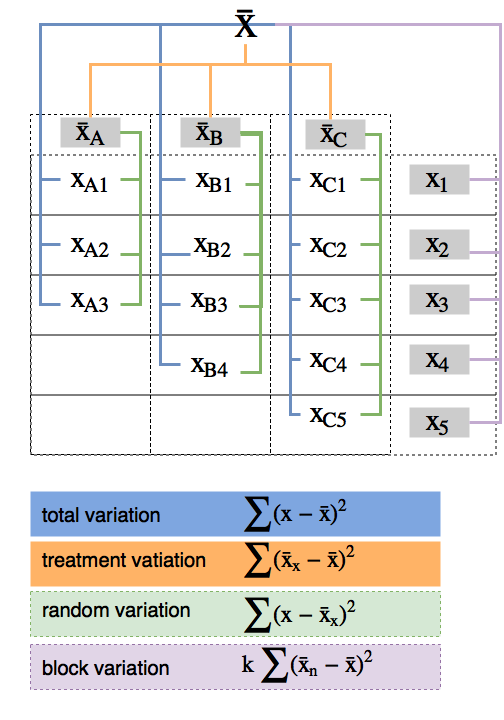
\includegraphics[width=0.3\textwidth]{./img/anova.png}
 \caption{Illustration of a Two-Way ANOVA}
 \label{fig:anova two-way illustration}
\end{center}
\end{figure} 
\hformbar

% insert new page to fit anova table
\newpage
\cleardoublepage


\formdesc{ANOVA: Two-Way with Interaction (Factors) -- Table} \\
\begin{equation}
\label{anova table two-way}
\centering \text{ANOVA Table with Interaction (Factors)}
\end{equation}
\begin{table}[!h] % position table exactly here
% \label{ANOVA table two-way}
 \begin{footnotesize} % squeeze text size of table
 \begin{tabular}{@{}lllll@{}}
 \toprule
 \multicolumn{5}{c}{ANOVA} \\
 \midrule
 source of variation & \multicolumn{1}{l}{SS} & \multicolumn{1}{c}{df} & \multicolumn{1}{l}{mean square} & \multicolumn{1}{c}{F} \\
 \midrule
 Factor A  & SSA & $k-1$ & $\frac{SSA}{(k-1)}=MSA$ & $\frac{MSA}{MSE}$ \\
 Factor B & SSB & $b-1$ & $\frac{SSB}{(b-1)}=MSB$ & $\frac{MSB}{MSE}$ \\
 Interaction & SSI & $(k-1)(b-1)$ & $\frac{SSI}{[(k-1)(b-1)]}=MSI$ & $\frac{MSI}{MSE}$ \\
 Error & SSE & $n-kb$ & $\frac{SSE}{(n-kb)} = MSE$ &  \\
 \multicolumn{1}{r}{total} & SS total  & $n - 1$ &  & 
 \end{tabular}
 \end{footnotesize}
\end{table}
\hformbar

% insert new page to fit anova table
\newpage
\cleardoublepage


\formdesc{Linear Regression: Correlation Coefficient}
\begin{equation}
\label{correlation coefficient}
r = \frac{\sum(x-\bar{x})(y-\bar{y})}{(n-1)s_{x}s_{y}}
\end{equation}
\textsc{Subject:} A measure of strength of the linear relationship between two variables. It ranges from $-1$ up to and including $+1$.

\textrm{Note:} The correlation coefficient becomes independent of the scale used if the term $\sum(x-\bar{x})(y-\bar{y})$ is divided by the sample standard deviations $s_{x}$ and $s_{y}$. Similarly, the term becomes independent of sample size once divided by $(n-1)$. 

\textrm{Note:} Correlation between two independent variables is considered uncritical if $-0.70 < r < 0.70$. A more precise test provides the variance inflation factor (VIF) as in formula \eqref{multiple regression variance inflation factor}.

where:
\begin{itemize}
 \item $r$ denotes the correlation coefficient.
 \item $x$ denotes the variable value of the x population.
 \item $y$ denotes the variable value of the y population.
 \item $\bar{x}$ denotes the mean of variable values in the x population.
 \item $\bar{y}$ denotes the mean of variable values in the y population.
 \item $n$ denotes the number of observations in the sample.
 \item $(n-1)$ denotes the degree of freedom.
 \item $s_{x}$ denotes the standard deviation of the x population.
 \item $s_{y}$ denotes the standard deviation of the y population.
\end{itemize}
\hformbar


\formdesc{Linear Regression: t Test for the Correlation Coefficient $r$}
\begin{equation}
\label{correlation coefficient t test}
t = \frac{r\sqrt{n-2}}{\sqrt{1-r^2}}
\end{equation}
\textsc{Subject:} Resolves the question about whether there could be zero correlation in the population from which the sample was selected.

with $n-2$ degrees of freedom where:
\begin{itemize}
 \item $r$ denotes the correlation coefficient.
 \item $n$ denotes the number of observations in the sample.
\end{itemize}
\hformbar


\formdesc{Linear Regression Equation: General Form}
\begin{equation}
\label{linear regression equation general form}
\hat{y} = a + bx
\end{equation}
\textsc{Subject:} An equation that expresses the linear relationship between two variables.

where:
\begin{itemize}
 \item $\hat{y}$ is the estimated value of the $y$ variable for a selected $x$ value.
 \item $a$ is the y-intercept. It is the estimated value of Y when $x = 0$.
 \item $b$ is the slope of the line, or the average change in $\hat{y}$ for each change of one unit (either increase or decrease) in the independent variable $x$.
 \item $x$ is any value of the independent variable that is selected.
\end{itemize}
\hformbar


\formdesc{Linear Regression: Slope of Regression Line}
\begin{equation}
\label{linear regression slope regression line}
b = r(\frac{s_{y}}{s_{x}})
\end{equation}
where:
\begin{itemize}
 \item $r$ denotes the correlation coefficient.
 \item $s_{y}$ denotes the standard deviation of y (the dependent variable).
 \item $s_{x}$ denotes the standard deviation of x (the independent variable).
\end{itemize}
\hformbar


\formdesc{Linear Regression: Y-Intercept}
\begin{equation}
\label{linear regression y intercept}
a = \bar{y} - b\bar{x}
\end{equation}
where:
\begin{itemize}
 \item $\bar{y}$ is the mean of y (the dependent variable).
 \item $\bar{x}$ is the mean of x (the independent variable).
\end{itemize}
\hformbar


\formdesc{Linear Regression: t Test for the Slope $b$}
\begin{equation}
\label{linear regression test slope}
t = \frac{b - 0}{s_{b}}
\end{equation}
\textsc{Subject:} Conducts a test on whether the slope of the regression line is different from zero. In such a circumstance we can reasonably conclude that the regression line adds to the predictive ability of the regression equation.

with $n-2$ degrees of freedom where:
\begin{itemize}
 \item $b$ is the estimate of the regression line's slope calculated from the sample information.
 \item $s_{b}$ is the standard error of the slope estimate, also determined from sample information.
\end{itemize}
\hformbar


\formdesc{Linear Regression: Standard Error of Estimate}
\begin{equation}
\label{linear regression standard error of estimate}
s_{y \cdotp x} = \sqrt{\frac{\sum(y-\hat{y})^2}{n-2}} = \sqrt{\frac{\text{SSE}}{n-2}}
\end{equation}
\textsc{Subject:} It is a relative measure of a regression equation's ability to predict.

where:
\begin{itemize}
 \item $s_{y \cdotp x}$ denotes the standard error of estimate with $y \cdotp x$ to be interpreted as the standard error of $y$ for a given value of $x$. It is the same concept as the standard deviation in formula \eqref{sample standard deviation} which measures the dispersion around a mean.
 \item $y$ denotes the observed value.
 \item $\hat{y}$ denotes the predicted value.
 \item $\sum(y-\hat{y})^2$ denotes the sum of squares error or residuals referred to in the ANOVA equation \eqref{anova table one-way} as $SSE$. 
\end{itemize}
\hformbar


\formdesc{Linear Regression: Coefficient of Determination}
\begin{equation}
\label{linear regression coefficient of determination}
r^2 = \frac{\text{SSR}}{\text{SS Total}} = \frac{\sum(\hat{y}-\bar{y})^2}{\sum(y-\bar{y})^2} =  1 - \frac{\text{SSE}}{\text{SS Total}} = 1 - \frac{\sum(y-\hat{y})^2}{\sum(y-\bar{y})^2}
\end{equation}
\textsc{Subject:} The proportion of the total variation in the dependent variable Y that is explained, or accounted for, by the variation in the independent variable X.

where:
\begin{itemize}
 \item \emph{SS Total} denotes total variation, that is, the sum of squares total.
 \item \emph{SSR} denotes the sum of squares regression.
 \item \emph{SSE} denotes the sum of squares errors or residuals, respectively.
\end{itemize}
\hformbar


\formdesc{Linear Regression: Confidence Interval for the Mean of Y given X}
\begin{equation}
\label{linear regression confidence interval}
\hat{y} \pm t s_{y \cdotp x}\sqrt{\frac{1}{n}+\frac{(x-\bar{x})^2}{\sum(x-\bar{x})^2}}
\end{equation}
\textsc{Subject:} Applied when the regression equation is used to predict the \emph{mean value of y} for a given value of x  

where:
\begin{itemize}
 \item $x$ denotes the given value.
 \item $\bar{x}$ denotes the sample mean.
 \item $\hat{y}$ denotes the predicted value. 
 \item $s_{y \cdotp x}$ denotes the standard error of estimate with $y \cdotp x$ to be interpreted as the standard error of $y$ for a given value of $x$. It is the same concept as the standard deviation in formula \eqref{sample standard deviation} which measures the dispersion around a mean.
\end{itemize}
\hformbar


\formdesc{Linear Regression: Prediction Interval for Y given X}
\begin{equation}
\label{linear regression prediction interval}
\hat{y} \pm t s_{y \cdotp x}\sqrt{1+\frac{1}{n}+\frac{(x-\bar{x})^2}{\sum(x-\bar{x})^2}}
\end{equation}
\textsc{Subject:} Applied when the regression equation is used to predict an \emph{individual value of y $(n = 1)$} for a given value of x. Refer to equation \eqref{linear regression confidence interval}.

where:
\begin{itemize}
 \item $x$ denotes the given value.
 \item $\bar{x}$ denotes the sample mean.
 \item $\hat{y}$ denotes the predicted value. 
 \item $s_{y \cdotp x}$ denotes the standard error of estimate with $y \cdotp x$ to be interpreted as the standard error of $y$ for a given value of $x$. It is the same concept as the standard deviation in formula \eqref{sample standard deviation} which measures the dispersion around a mean.
\end{itemize}
\hformbar


\formdesc{Multiple Regression: General Equation}
\begin{equation}
\label{multiple regression general equation}
\hat{y} = a + b_{1}x_{1} + b_{2}x_{2} + b_{3}x_{3} + ... b_{k}x_{k}
\end{equation}
\textsc{Subject:} Enhanced equation of formula \eqref{linear regression equation general form} for more than one dependent variable.

where:
\begin{itemize}
 \item $a$ is the intercept, the value of $\hat{y}$ when all the x's are zero.
 \item $b_{j}$ is the amount by which $\hat{y}$ changes when that particular $x_{j}$ increases by one unit, with the values of all other independent variables held constant.
 \item $k$ represents the number of independent variables.
\end{itemize}
\hformbar


\formdesc{Multiple Regression: Standard Error of Estimate}
\begin{equation}
\label{multiple regression standard error of estimate}
s_{y \cdotp 123 \cdotp k} = \sqrt{\frac{\sum(y-\hat{y})^2}{n-(k+1)}} = \sqrt{\frac{\text{SSE}}{n-(k+1)}} = \sqrt{\text MSE}
\end{equation}
\textsc{Subject:} It is a relative measure of a regression equation's ability to predict for more than one independent variable.

where:
\begin{itemize}
 \item $y$ is the actual observation.
 \item $\hat{y}$ is the estimated value computed from the regression equation.
 \item $n$ is the number of observations in the sample.
 \item $k$ is the number of independent variables.
 \item $SSE$ is the residual sum of squares from an ANOVA table. It is equal to the term $\sum(y-\hat{y})^2$ as used also in the ANOVA formula \eqref{anova table one-way}. 
\end{itemize}
\hformbar


\formdesc{Multiple Regression ANOVA -- Table} \\
\begin{equation}
\label{multiple regression anova table}
\centering \text{Multiple Regression ANOVA Table}
\end{equation}
\begin{table}[!h] % position table exactly here
% \label{Multiple Regression ANOVA Table}
 \begin{footnotesize} % squeeze text size of table
 \begin{tabular}{@{}lllll@{}}
 \toprule
 \multicolumn{5}{c}{ANOVA} \\
 \midrule
 source & \multicolumn{1}{l}{SS} & \multicolumn{1}{c}{df} & \multicolumn{1}{l}{MS} & \multicolumn{1}{c}{F} \\
 \midrule
 Regression  & SSR & $k$ & $MSR = \frac{SSR}{k}$ & $\frac{MSR}{MSE}$ \\
 Residual or error & SSE & $n-(k+1)$ & $MSE = \frac{SSE}{n-(k+1)}$ & $$ \\
 \multicolumn{1}{r}{total} & SS total  & $n - 1$ &  & 
 \end{tabular}
 \end{footnotesize}
\end{table}
\hformbar


\formdesc{Multiple Regression: Coefficient of Multiple Determination}
\begin{equation}
\label{multiple regression coefficient of multiple determination}
R^2 = \frac{\text{SSR}}{\text{SS Total}}
\end{equation}
\textsc{Subject:} The percent of variation in the dependent variable, $y$, explained by the set of independent variables, $x_{1}$, $x_{2}$, $x_{3}$, ... $x_{k}$.

where:
\begin{itemize}
 \item \emph{SS Total} denotes total variation, that is, the sum of squares total.
 \item \emph{SSR} denotes the sum of squares regression.
\end{itemize}
\hformbar


\formdesc{Multiple Regression: Adjusted Coefficient of Multiple Determination}
\begin{equation}
\label{multiple regression adjusted coefficient of multiple determination}
R^2_{adj} = \frac{\frac{SSE}{n-(k+1)}}{\frac{\text SS total}{n-1}}
\end{equation}
\textsc{Subject:} The percent of variation in the dependent variable, $y$, explained by the set of independent variables, $x_{1}$, $x_{2}$, $x_{3}$, ... $x_{k}$. As more independent variables are added to the multiple regression model $R^2$ of formula \eqref{multiple regression coefficient of multiple determination} tends to increase. In fact, if the number of variables, $k$, and the sample size, $n$, are equal, the coefficient of determination is 1. To avoid this trend $R^2$ is adjusted. 

where:
\begin{itemize}
 \item \emph{SS Total} denotes total variation, that is, the sum of squares total.
 \item \emph{SSE} denotes the sum of squares error or residual.
\end{itemize}
\hformbar


\formdesc{Multiple Regression: Global Test}
\begin{equation}
\label{multiple regression global test}
F = \frac{\frac{\text SSR}{k}}{\frac{\text SSE}{n-(k+1)}}
\end{equation}
\textsc{Subject:} The Global Test investigates whether it is possible all the independent variables have zero regression coefficients. As in formula \eqref{critical value for f statistic} it expresses this as sum of squares regression per unit of sum of squares residuals. The higher the explained variances compared to the residual variances, the more positive the value of the F distribution.

where:
\begin{itemize}
 \item \emph{SSR} denotes the sum of squares regression.
 \item \emph{SSE} denotes the sum of squares error or residual.
 \item $n$ is the number of observations in the sample.
 \item $k$ is the number of independent variables.
\end{itemize}
\hformbar


\formdesc{Multiple Regression: t Test Individual Coefficients $b$}
\begin{equation}
\label{multiple regression t test individual coefficients}
t = \frac{b_{j} - 0}{s_{b_{j}}}	
\end{equation}
\textsc{Subject:} Conducts a test on the independent variables individually to determine whether the regression coefficients differ from zero. If a regression coefficient is likely to be zero it does not contribute to the regression equation's ability to predict. 

where:
\begin{itemize}
 \item $b_{j}$ refers to any one of the regression coefficients.
 \item $s_{b}$ is the standard error of the slope estimate, also determined from sample information.
\end{itemize}
\hformbar


\formdesc{Multiple Regression: Variance Inflation Factor}
\begin{equation}
\label{multiple regression variance inflation factor}
VIF = \frac{1}{1 - R^2_{j}}
\end{equation}
\textsc{Subject:} A VIF greater than 10 is considered unsatisfactory, indicating that the independent variable should be removed from the analysis.

where:
\begin{itemize}
 \item $R^2_{j}$ refers to the coefficient of determination
\end{itemize}
\hformbar


\formdesc{Test of Hypothesis: One Proportion}
\begin{equation}
\label{test hypothesis one proportion}
z = \frac{p - \pi}{\sqrt{\frac{\pi(1 - \pi)}{n}}}
\end{equation}

where:
\begin{itemize}
 \item $\pi$ is the population proportion.
 \item $p$ is the sample proportion.
 \item $n$ is the sample size.
\end{itemize}
\hformbar


\formdesc{Test of Hypothesis: Pooled Proportion}
\begin{equation}
\label{test hypothesis pooled proportion}
p_c = \frac{x_1 + x_2}{n_1 + n_2}
\end{equation}

where:
\begin{itemize}
 \item $p_{c}$ is the pooled proportion possessing the trait in the combined samples. It is called the pooled estimate of the population proportion.
 \item $x_1$ is the number possessing the trait in the first sample.
 \item $x_2$ is the number possessing the trait in the second sample.
 \item $n_{1}$ is the number of observations in the first sample.
 \item $n_{2}$ is the number of observations in the second sample.
 \end{itemize}
\hformbar


\formdesc{Test of Hypothesis: Two-Sample Test of Proportions}
\begin{equation}
\label{test hypothesis two sample test proportion}
z = \frac{p_{1} - p_{2}}{\sqrt{\frac{p_{c}(1 - p_{c})}{n_{1}}} + \frac{p_{c}(1 - p_{c})}{n_{2}}}
\end{equation}

where:
\begin{itemize}
 \item $n_{1}$ is the number of observations in the first sample.
 \item $n_{2}$ is the number of observations in the second sample.
 \item $p_{1}$ is the proportion in the first sample possessing the trait.
 \item $p_{2}$ is the proportion in the second sample possessing the trait.
 \item $p_{c}$ is the pooled proportion possessing the trait in the combined samples. It is called the pooled estimate of the population proportion.
\end{itemize}
\hformbar


\formdesc{Chi-Square Test Statistic}
\begin{equation}
\label{test hypothesis chi square test statistic}
\chi^2 = \sum\left[\frac{(f_o - f_e)^2}{f_e}\right]
\end{equation}

with $k - 1$ degrees of freedom, where:
\begin{itemize}
 \item $k$ is the number of categories.
 \item $f_o$ is an observed frequency in a particular category.
 \item $f_e$ is an expected frequency in a particular category.
 \end{itemize}
\hformbar


\formdesc{Expected Frequency}
\begin{equation}
\label{expected frequency}
f_e =  \frac{\text{(row total) \text{(column total)}}}{\text{(grand total)}}
\end{equation}

where:
\begin{itemize}
 \item $f_e$ is an expected frequency in a particular category.
 \end{itemize}
\hformbar


\formdesc{Sign Test: n $>$ 10}
\begin{equation}
\label{sign text n > 10}
z = \frac{(x \pm .50) - \mu}{\sigma}
\end{equation}

where:
\begin{itemize}
 \item $z$ refers to the standard value.
 \item $\pm 0.50$ is the \emph{continuity correction factor} as in formula \eqref{continuity correction factor}.
 \item $x$ denotes the number of plus ($+$) or minus ($-$) signs. 
 \item $\mu$ denotes the population mean.
 \item $\sigma$ denotes the population standard deviation.
 \end{itemize}
\hformbar


\formdesc{Sign Test: n $>$ 10, + Signs \emph{more} than $n/2$}
\begin{equation}
\label{sign text n > 10 + signs more}
z = \frac{(x - .50) - \mu}{\sigma} = \frac{(x - .50) - .50n}{.50\sqrt{n}}
\end{equation}

where:
\begin{itemize}
 \item $z$ refers to the standard value.
 \item $\pm 0.50$ is the \emph{continuity correction factor} as in formula \eqref{continuity correction factor}.
 \item $x$ denotes the number of plus ($+$) or minus ($-$) signs.
 \item $n$ denotes the sample size.
 \item $\mu$ denotes the population mean.
 \item $\sigma$ denotes the population standard deviation.
 \end{itemize}
\hformbar


\formdesc{Sign Test: n $>$ 10, + Signs \textbf{less} than $n/2$}
\begin{equation}
\label{sign text n > 10 + signs less}
z = \frac{(x + .50) - \mu}{\sigma} = \frac{(x + .50) - .50n}{.50\sqrt{n}}
\end{equation}

where:
\begin{itemize}
 \item $z$ refers to the standard value.
 \item $\pm 0.50$ is the \emph{continuity correction factor} as in formula \eqref{continuity correction factor}.
 \item $x$ denotes the number of plus ($+$) or minus ($-$) signs.
 \item $n$ denotes the sample size.
 \item $\mu$ denotes the population mean.
 \item $\sigma$ denotes the population standard deviation.
 \end{itemize}
\hformbar


\formdesc{Wilcoxon Rank-Sum Test}
\begin{equation}
\label{wilcoxon rank sum test}
z = \frac{W - \frac{n_1(n_1 + n_2 + 1)}{2}}{\sqrt{\frac{n_1n_2(n_1 + n_2 + 1)}{12}}}
\end{equation}
\textsc{Subject:} this test is specifically designed to determine whether two \emph{independent samples} came 
from equivalent populations.

Note: this test is an alternative to the Two-Sample t test as in formula \eqref{two-sample test of means sigma unknown}, however it does \textbf{not} require that the two populations follow the normal distribution and have equal population variances.

where:
\begin{itemize}
 \item $n_1$ is the number of observations of the first population.
 \item $n_2$ is the number of observations of the second population.
 \item $W$ is the sum of the ranks from the first population.
\end{itemize}
\hformbar


\formdesc{Kruskal-Wallis Test}
\begin{equation}
\label{kruskal wallis test}
H = \frac{12}{n(n + 1)}\left[\frac{(\sum R_1)^2}{n_1} + \frac{(\sum R_2)^2}{n_2} + ... + \frac{(\sum R_k)^2}{n_k}\right] - 3(n+1) 
\end{equation}
Note: for the Kruskal-Wallis test to be applied, the samples selected from the populations must be independent. If in addition the following prerequisites are met an ANOVA analysis as in formula \eqref{anova components} can be applied instead:
\begin{itemize}
 \item The samples are from independent populations.
 \item The population variances must be equal.
 \item The samples are from normal populations.
\end{itemize}

with $k-1$ degrees of freedom ($k$ is the number of populations), where:
\begin{itemize}
 \item $\sum R_1, \sum R_2, ..., \sum R_k$ are the sums of the ranks of samples 1, 2, ... k, respectively.
 \item $n_1, n_2, ..., n_k$ are the sizes of samples 1, 2, ..., k, respectively.
 \item $n$ is the combined number of observations for all samples.
\end{itemize}
\hformbar


\formdesc{Spearman's Coefficient of Rank Correlation}
\begin{equation}
\label{spearman coefficient}
r_s = 1 - \frac{6\sum d^2}{n(n^2 - 1)}
\end{equation}

where:
\begin{itemize}
 \item $r_s$ is Spearman's coefficient of rank correlation.
 \item $d$ is the difference between the ranks for each pair.
 \item $n$ is the number of paired observations.
\end{itemize}
\hformbar


\formdesc{Hypothesis Test: Rank Correlation}
\begin{equation}
\label{hypothesis rank correlation}
t = r_s\sqrt{\frac{n - 2}{1 - r_s^2}}
\end{equation}

where:
\begin{itemize}
 \item $r_s$ is Spearman's coefficient of rank correlation.
\end{itemize}
\hformbar


\formdesc{Index Numbers: Simple Index}
\begin{equation}
\label{simple index}
P = \frac{p_t}{p_0}*100
\end{equation}

where:
\begin{itemize}
 \item $p_0$ is the base-period price.
 \item $p_t$ is the given period price.
\end{itemize}
\hformbar


\formdesc{Index Numbers: Simple Average of the Price Relatives}
\begin{equation}
\label{simple average of the price relatives}
P = \frac{\sum P_i}{n}
\end{equation}
Note: 
\begin{itemize}
 \item Advantage: simple price indices are not dependent on the unit of measure of the item quantified.
 \item Disadvantage: simple price indices do not the account for the relative importance of the items included.
\end{itemize}
The aforementioned shortcomings of not accounting for the relative importance, i.e. the marginal quantities consumed in each item category, are mitigated by the Laspeyres price index as in formula \eqref{laspeyres price index} and the Paasche price index as in formula \eqref{paasche price index}.

where:
\begin{itemize}
 \item $P_i$ refers to the simple index for each to the items.
 \item $n$ refers to the number of items. 
\end{itemize}
\hformbar


\formdesc{Index Numbers: Simple Aggregate Index}
\begin{equation}
\label{simple aggregate index}
P = \frac{\sum p_t}{\sum p_0}*100
\end{equation}
Note: since the aggregate index is influenced by the unit of measure, it is not used frequently.

where:
\begin{itemize}
 \item $p_0$ is the base-period price.
 \item $p_t$ is the given period price. 
\end{itemize}
\hformbar


\formdesc{Index Numbers: Laspeyres Price Index}
\begin{equation}
\label{laspeyres price index}
P = \frac{\sum p_t q_0}{\sum p_0 q_0}*100
\end{equation}
Note: the Laspeyres price index thus assumes that the base period quantities have still important bearing on the current price index and thus are realistic. Hence it contrasts the assumption of the Paasche price index as in formula \eqref{paasche price index}.

where:
\begin{itemize}
 \item $P$ is the price index.
 \item $p_t$ is the current price.
 \item $p_0$ is the price in the base period.
 \item $q_0$ is the quantity used in the base period.
\end{itemize}
\hformbar


\formdesc{Index Numbers: Paasche Price Index}
\begin{equation}
\label{paasche price index}
P = \frac{\sum p_t q_t}{\sum p_0 q_t}*100
\end{equation}
Note: the Paasche price index assumes current period quantity levels as base to account for changed preferences in consumed quantities. Hence, it contrasts the assumption of the Laspeyres price index as in formula \eqref{laspeyres price index}.

where:
\begin{itemize}
 \item $P$ is the price index.
 \item $p_t$ is the current price.
 \item $p_0$ is the price in the base period.
 \item $q_0$ is the quantity used in the base period.
\end{itemize}
\hformbar


\formdesc{Index Numbers: Fisher's Ideal Index}
\begin{equation}
\label{fisher ideal index}
\text{Fisher's Ideal Index} = \sqrt{\text{(Laspeyres index)}\text{(Paasche index)}}
\end{equation}
Note: Fisher's Ideal Index is actually a geometric mean \eqref{geometric mean} of Laspeyres \eqref{laspeyres price index} and Paasche \eqref{paasche price index} price indices.
\hformbar


\formdesc{Index Numbers: Value Index}
\begin{equation}
\label{value index}
V = \frac{\sum p_t q_t}{\sum p_0 q_0}*100
\end{equation}

where:
\begin{itemize}
 \item $P$ is the price index.
 \item $p_t$ is the current price.
 \item $p_0$ is the price in the base period.
 \item $q_0$ is the quantity used in the base period.
\end{itemize}
\hformbar


\formdesc{Index Numbers: Real Income}
\begin{equation}
\label{real income}
\text{Real income} = \frac{\text{Money income}}{\text{CPI}}*100
\end{equation}

where:
\begin{itemize}
 \item $CPI$ denotes consumer price index.
\end{itemize}
\hformbar


\formdesc{Index Numbers: Index as a Deflator}
\begin{equation}
\label{index deflator}
\text{Deflated sales} = \frac{\text{Actual sales}}{\text{An appropriate index}}*100
\end{equation}
\hformbar


\formdesc{Index Numbers: Index for Purchasing Power}
\begin{equation}
\label{purchasing power}
\text{Purchasing power of dollar} = \frac{\text{\$1}}{\text{CPI}}*100
\end{equation}
\hformbar



\formdesc{Time Series \& Forecasting: Linear Trend Equation}
\begin{equation}
\label{linear trend equation}
\hat{y} = a + bt
\end{equation}

where:
\begin{itemize}
 \item $\hat{y}$ is the projected value of the $y$ variable for a selected value of $t$.
 \item $a$ is the y-intercept. It is the estimated value of y when $t = 0$.
 \item $b$ is the slope of the line, or the average change in $\hat{y}$ for each increase of one unit in $t$.
 \item $t$ is any value of time that is selected.
\end{itemize}
\hformbar


\formdesc{Time Series \& Forecasting: Log Trend Equation}
\begin{equation}
\label{log trend equation}
\log \hat{y} = \log a + \log b(t)
\end{equation}
\hformbar


\formdesc{Time Series \& Forecasting: Correction Factor for Adjusting Quarterly Means}
\begin{equation}
\label{correction factor adjusting quarterly means}
\text{Correction factor} = \frac{4.00}{\text{Total of four means}}
\end{equation}
\hformbar


\formdesc{Time Series \& Forecasting: Durbin-Watson Statistic}
\begin{equation}
\label{durbin-watson statistic}
d = \frac{\sum_{t = 2}^{n} (e_t - e_{t-1})^2}{\sum_{t = 1}^n(e_t)^2}  
\end{equation}
\hformbar

\end{document}